\documentclass[../Cover.tex]{subfiles}

\begin{document}
	\begin{minipage}[t][0.2\textheight][t]{0.1\textwidth} 
		
\includegraphics[width=\textwidth]{DC.png}
	\end{minipage}
	\hfill
	\begin{minipage}[t][0.2\textheight][t]{0.8\textwidth}
		\begin{tabular}{ p{0.25\textwidth} l  }		
			\\	
			\textbf{Box Drill} \\
			\\[0.09\textheight]
		\end{tabular}
		\quad
		%%%%%%%%%%%%%%%%%%%%%%%%%%%
		% Quick Facts Table       %
		%%%%%%%%%%%%%%%%%%%%%%%%%%%
		\begin{tabular}{ | p{0.2\textwidth} | p{0.2\textwidth} | p{0.1\textwidth} |}
			\hline
			\rowcolor[HTML]{C0C0C0}\tiny Weapon Type & \tiny Distance & \tiny Par Time\\ 
			\hline
			\tiny Pistol/Long arm & \tiny 7-10yd/15-25yd & \tiny 8s \\ % EDIT HERE
			\hline
		\end{tabular}
	\end{minipage}
	%%%%%%%%%%%%%%%%%%%%%%%%%%%
	% Requirements      %
	%%%%%%%%%%%%%%%%%%%%%%%%%%%
	\begin{tabular}{p{0.25\textwidth}}
		\small Requirements \\
		\hline
		\tiny \begin{itemize} % EDIT HERE
			\item Target type: 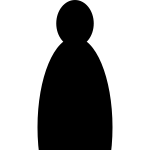
\includegraphics[width=0.03\textwidth]{body-target.png}
			\item 2 Targets, 1 yard apart
			\item 2 3x5" index cards
			\item Rounds Fired: 6
			\item Starting Position: Any
		\end{itemize}
		
		\tikzset{every picture/.style={line width=0.75pt}} %set default line width to 0.75pt        
		
		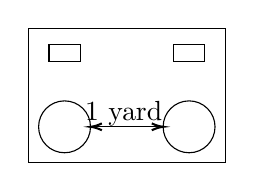
\begin{tikzpicture}[x=0.75pt,y=0.75pt,yscale=-0.5,xscale=0.5]
			%Shape: Circle [id:dp4972510664234988] 
			\draw   (250,145) .. controls (250,131.19) and (261.19,120) .. (275,120) .. controls (288.81,120) and (300,131.19) .. (300,145) .. controls (300,158.81) and (288.81,170) .. (275,170) .. controls (261.19,170) and (250,158.81) .. (250,145) -- cycle ;
			%Shape: Circle [id:dp4355053162856828] 
			\draw   (370,145) .. controls (370,131.19) and (381.19,120) .. (395,120) .. controls (408.81,120) and (420,131.19) .. (420,145) .. controls (420,158.81) and (408.81,170) .. (395,170) .. controls (381.19,170) and (370,158.81) .. (370,145) -- cycle ;
			%Shape: Rectangle [id:dp7012640745946925] 
			\draw   (260,66) -- (290,66) -- (290,82) -- (260,82) -- cycle ;
			%Shape: Rectangle [id:dp8235424935315838] 
			\draw   (380,66) -- (410,66) -- (410,82) -- (380,82) -- cycle ;
			%Straight Lines [id:da28167137742303594] 
			\draw    (302,145) -- (368,145) ;
			\draw [shift={(370,145)}, rotate = 180] [color={rgb, 255:red, 0; green, 0; blue, 0 }  ][line width=0.75]    (10.93,-3.29) .. controls (6.95,-1.4) and (3.31,-0.3) .. (0,0) .. controls (3.31,0.3) and (6.95,1.4) .. (10.93,3.29)   ;
			\draw [shift={(300,145)}, rotate = 0] [color={rgb, 255:red, 0; green, 0; blue, 0 }  ][line width=0.75]    (10.93,-3.29) .. controls (6.95,-1.4) and (3.31,-0.3) .. (0,0) .. controls (3.31,0.3) and (6.95,1.4) .. (10.93,3.29)   ;
			%Shape: Rectangle [id:dp23844923414397856] 
			\draw   (240,50) -- (430,50) -- (430,179) -- (240,179) -- cycle ;
			
			% Text Node
			\draw (332,132) node  [align=left] {1 yard};
		\end{tikzpicture}
			
		\\[0.6\textheight]
	\end{tabular}
	% Steps and Scoring	
	\begin{tabular}{ | p{0.65\textwidth} |}
		\hline
		%%%%%%%%%%%%%%%%%%%%%%%%%%%
		% Steps                   %
		%%%%%%%%%%%%%%%%%%%%%%%%%%%
		\rowcolor[HTML]{C0C0C0}Steps\\ 
		\hline
		\tiny \begin{enumerate}[topsep=0pt, partopsep=0pt]
			\item Attach one index card at approx. eye level on each target. Place an 8" circle target in the center mass.
			\item On the start signal, fire two rounds at the left target's center mass, then two on the right target's center mass (8" circle).
			\item Assess the situation.
			\item Fire one round in the right target's head (index card) and one in the left target's head.
		\end{enumerate}		
		\\ [0.25\textheight]
		\hline
		%%%%%%%%%%%%%%%%%%%%%%%%%%%
		% Scoring                 %
		%%%%%%%%%%%%%%%%%%%%%%%%%%%
		\rowcolor[HTML]{C0C0C0}Scoring \\
		\hline
		\tiny \begin{itemize}[topsep=0pt, partopsep=0pt]
			\item Center mass hits are 5pts (8" circle). Head hits are 10 pts (index card).
			\item For an added challenge, swap the 8" circles for 3x5" index cards.
			\item For an added challenge, have a partner signal step 4.
			\item Passing Hit Factor: 5.0 
		\end{itemize}		
		\\ [0.2\textheight]
		\hline
	\end{tabular}
\end{document}
